\section{Introduction}
Through this chapter research will be conducted into varying areas related to the project. The conclusions made from 
this research will support any design or implementation decisions made in the course of the project.
\section{The Binding of Isaac}
`The Binding of Isaac: Rebirth is a randomly generated action RPG shooter with heavy Rogue-like elements.'\cite*{BindingIsaacRebirtha}
The player progresses through 'floors' which are made up of a series of 'rooms', each room can contain a variety of enemies, traps, and items.
Each floor has a set of 'special rooms', namely a boss room, item room and a shop. The goal is to use the items found on each floor to defeat each boss,
progressing to the next floor until the game is finished. The items in the game often interact, this interaction is usually called a 'synergy' if it benefits the player.
In this instance the rogue-like elements are that the game has to be successfully completed many times, these are called 'runs'. Each run is unique and depending on the 
actions the player takes in the run it can have different outcomes and more parts of the game can be unlocked.
\section{Existing Solutions}
While there is no existing solution that is a direct comparison to this project, there are applications that have a 
similar purpose. These will be analysed to determine what features should also be implemented in this project and what 
could be improved by this project.
\subsection*{Fandom Wiki}
\begin{figure}[H]
    \centering
    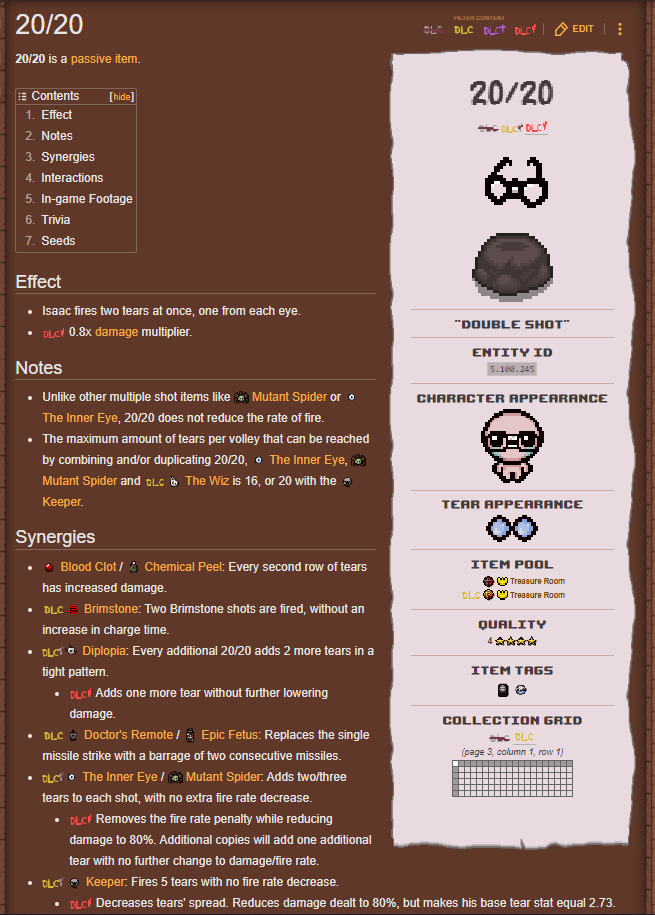
\includegraphics[width=0.8\textwidth]{wiki}
    \caption{Item page from Fandom Wiki}
\end{figure}
The Binding of Isaac has two wiki sites hosted on the Fandom Wiki platform; one for the original flash 
game\cite{BindingIsaacWiki}, and one for the modern version, commonly referred to as 'Rebirth'\cite{BindingIsaacRebirth}.
For the purposes of this project we will only be considering the modern version as it is widely considered the 'goto' 
version within the game's community.\par The website contains comprehensive information on all aspects of the game, 
and it is continually updated by the community. Users can navigate the site using either predefined categories or a 
powerful search tool. \par
Advantages
\begin{itemize}
    \item Contains information on all aspects of the game
    \item Actively maintained by the community
    \item Useful search functionality
\end{itemize}
Disadvantages
\begin{itemize}
    \item So much information can make it hard to find what is relevant
    \item Unable to search for interactions, have to go via each item 
\end{itemize}
\subsection*{Platinum God}
\begin{figure}[H]
    \centering
    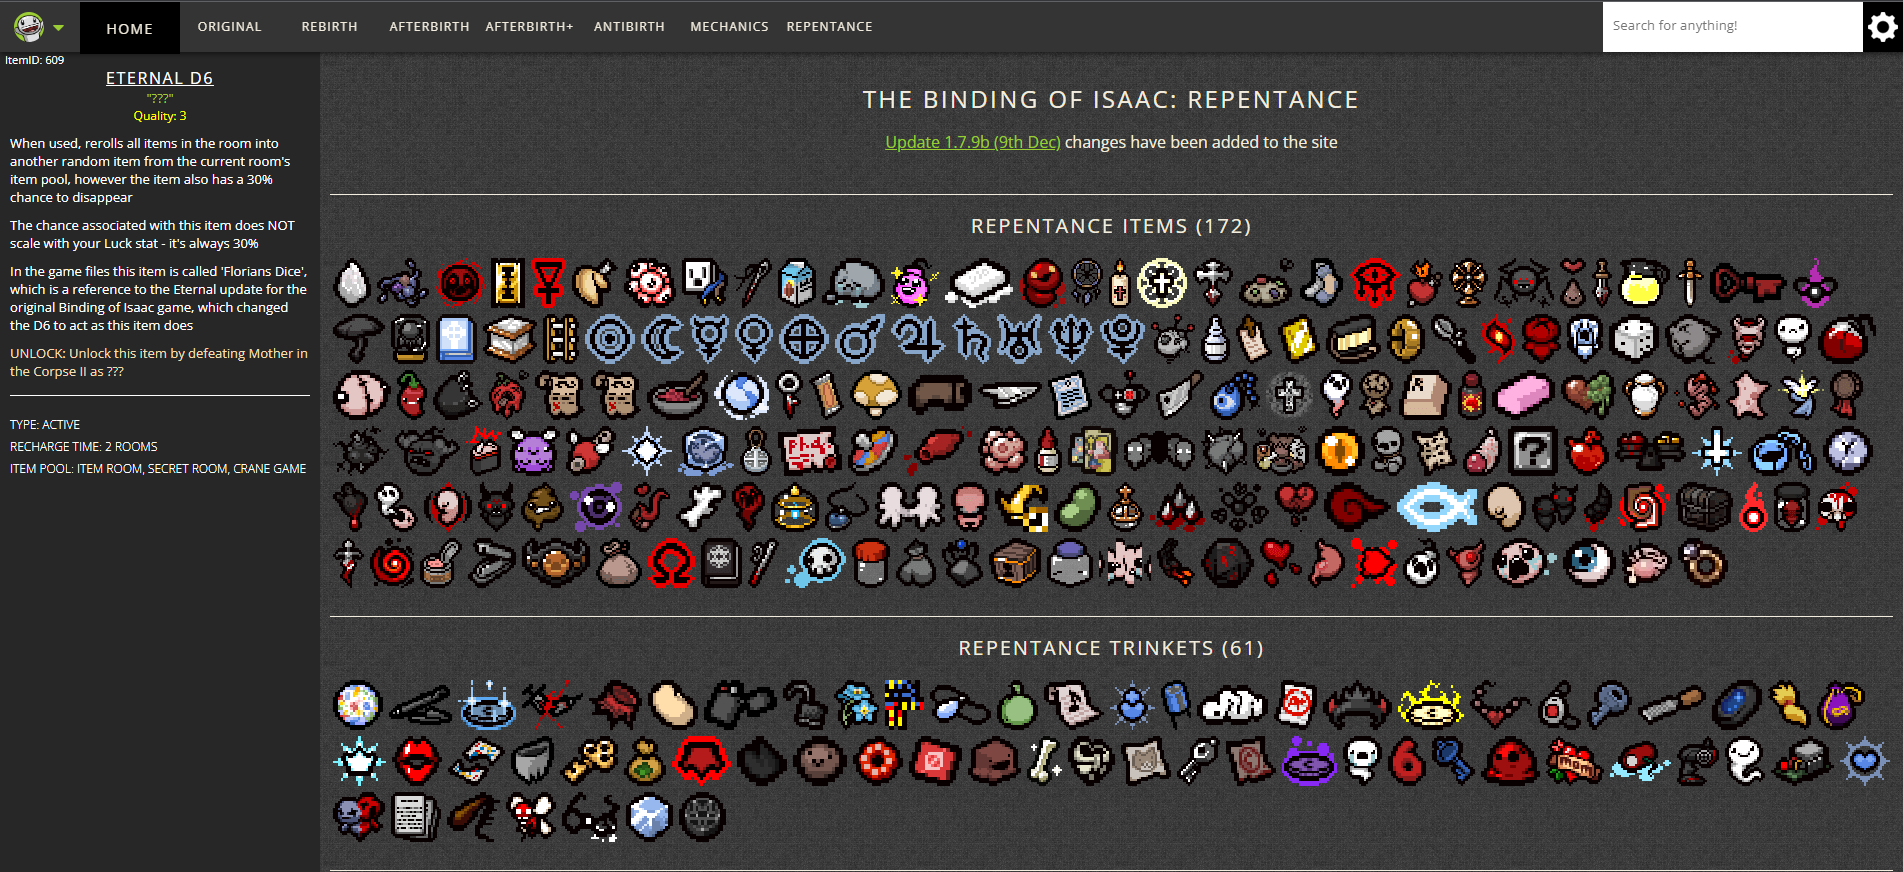
\includegraphics[width=0.8\textwidth]{platgod}
    \caption{Platinum God main page}
\end{figure}
Platinum God is a self-described `Isaac Cheat Sheet'\cite{IsaacCheatSheet}, and it contains item and key mechanic 
information for all versions of the game. The site is maintained by one person, and it claims to be more accurate than 
the community wiki as its updates are `tested thoroughly in the game using Cheat Engine'\cite{FrequentlyAskedQuestions}. 
The information is split into pages based on the version of the game; users can navigate this using the item icons which
 are arrayed on the page, or by using the search functionality. The search tool has some supported keywords, but will 
still usually require entering an exact match to an entry in the data. For certain versions of the game there is also a 
synergy finder tool which lets the user enter two items to see how they interact. However, this is limited to older 
versions of the game and only a small set of the items are actually included in the tool. \par
Advantages
\begin{itemize}
    \item Information is more reliable than the community wiki
    \item Easier to reference quickly due to there being less information
\end{itemize}
Disadvantages
\begin{itemize}
    \item Only one maintainer can mean long update times
    \item Only contains basic information about each item
    \item Limited or no synergy information for most items
    \item Harder to find items without knowing the name or what the item looks like
\end{itemize}
\section{Technology Review}
This section will research the potential technologies for the project and conclude with decisions about each.
\subsection{Client Side Framework}
\subsubsection*{Angular}
`Angular is an application-design framework and development platform for creating efficient and sophisticated 
single-page apps.'\cite{AngularIntroductionAngular} It was developed by Google to provide a complete framework for 
simple to complex single-page apps. Due to the size of this framework and the fact that it utilises Typescript makes for
 a steep learning curve, however this is counteracted by the large number of resources available from it being hugely 
popular and backed by a large company.
\subsubsection*{React}
`React is a declarative, efficient, and flexible JavaScript library for building user interfaces. It lets you compose 
complex UIs from small and isolated pieces of code called “components”.'\cite{TutorialIntroReact} React allows the 
developer to use JSX to combine HTML and JavaScript into one file, although this is not required to benefit from React. 
Unlike Angular, this is a library and not a full framework. This will reduce the amount of learning required to use it,
but it is likely extra libraries will be required to provide all the functionality required. There is also a lot of 
resources available as React is maintained by Meta and is the most popular of the frameworks considered according the 
2022 Stack Overflow Developer Survey\cite{StackOverflowDeveloper}.
\subsubsection*{Vue}
`An approachable, performant and versatile framework for building web user interfaces.'\cite{VueJsProgressive} While not
 backed by a large company, Vue has grown in popularity and has many large commercial sponsors. This means there is 
likely to be less documentation available, but this library is relatively simple compared to the options considered 
above. 
\subsubsection*{Conclusion}
After reviewing the three frameworks, the decision was made to use Angular for the project. This is due to prior 
experience with the framework, and with no background in JavaScript the increase in learning curve from Typescript is 
negligible. However, any of these choices would have been suitable for the project and the decision is mostly down to 
personal preference.
\subsection{Server Side Framework}
Due to the previously mentioned lack of JavaScript experience, the decision was made to only consider Python based 
frameworks to reduce the number of languages to learn.
\subsubsection*{Django}
`Django is a high-level Python web framework that encourages rapid development and clean, pragmatic design.'\cite{Django}
As with Angular, this can be used as a full framework and so, while it will contain almost everything required, there 
will also be a lot of unnecessary features included. Django was designed to support rapid development, as shown by the 
slogan `The web framework for perfectionists with deadlines.'\cite{Django}. It features database abstraction which
 allows developers to create `Models' to represent the data stored in a database, handling communication with the 
database avoiding the need for coding in SQL.
\subsubsection*{Flask}
`Flask is a lightweight WSGI web application framework.'\cite{ronacherFlaskSimpleFramework} It is a micro-framework that
 started as a wrapper for Jinja and Werkzeug and has grown into a popular web framework. Flask does not provide much 
functionality that is already provided by another extension, this keeps Flask small but can introduce complex library 
requirements. 
\subsubsection*{Conclusion}
Django was chosen here, again due to prior experience, particularly in using Django and Angular together. While using 
two large frameworks may result in the project suffering from an amount of bloat, the prior experience means completing
 the project and having time to refine it is more likely.
\subsection{Database}
A graph database is a type of NoSQL database that uses nodes, edges, and properties to represent and store data. It is 
often described as storing data as it would be drawn on a whiteboard. This approach makes querying relationships in the 
data much faster as they are embedded in the data, rather than using JOIN operations or cross lookups often seen in SQL 
implementations. The underlying storage mechanism of a graph database can vary, some depending on an abstraction to store
 the data in a typical table based manner and some opting for a `native' approach, maintaining the graph structure 
throughout the system.
\subsubsection*{Neo4j}
`Neo4j is an open-source, NoSQL, native graph database that provides an ACID-compliant transactional backend for your 
applications'\cite{WhatGraphDatabasea} Neo4j provide various tools for developing with graph databases, only the Aura 
platform will be considered here as it is the direct comparison for the other tools discussed, and a managed service is 
ideal for this project. A free database instance is provided in AuraDB for each account which allows up to 200000 nodes
 and 400000 relationships. Aura features a data import tool that allows developers to create a model of the database 
structure which can then be populated with data from CSV files. It also has an explore tool, Bloom, this allows 
developers to view the database graphically and queries can be performed to show expected outputs. Neo4j provide a lot 
of useful documentation and tutorials for all the services they provide, this includes free e-books and course style 
content to guide users through the material.
\subsubsection*{Amazon Neptune}
`Amazon Neptune is a purpose-built, high-performance graph database engine optimized for storing billions of 
relationships and querying the graph with milliseconds latency.'\cite{WhatGraphDatabase} Neptune is a managed graph 
database service provided by AWS. It offers a high throughput and low latency system that automatically scales with 
demand. As to be expected from any AWS product it is also highly secure and fault-tolerant. However, this comes at a 
cost; a free trial is offered for 30 days and after that a monthly fee is incurred with additional costs for data 
transfer, backups, and storage consumption.
\subsubsection*{Conclusion}
The decision was made to use Neo4j. This is primarily because the Aura platform provides a permanent free database 
instance which has ample resources for this project. There also exists a Python libraries, neomodel and django-neomodel,
 for easily integrating database access using Django Models. 
\section{Conclusion}
Throughout this chapter research has been conducted that will continue to provide benefit throughout the design and 
implementation stages. The review of existing solutions has highlighted the need for this application and has provided 
insight into how existing solutions have addressed the issue. The technology review has made it clear which technologies
 should be taken forward in the project as well as providing some background on why these technologies are needed and 
how they work.